\documentclass[conference]{IEEEtran}
\IEEEoverridecommandlockouts

\usepackage[T1]{fontenc}
\usepackage[utf8]{inputenc}
\usepackage{cite}
\usepackage{amsmath,amssymb}
\usepackage{graphicx}
\usepackage{booktabs}
\usepackage{xcolor}
\usepackage{microtype}
\usepackage{tikz}
\usetikzlibrary{arrows.meta,positioning,calc}
\usepackage[hidelinks]{hyperref}
\usepackage{url}
\usepackage{balance}

\def\BibTeX{{\rm B\kern-.05em{\sc i\kern-.025em b}\kern-.08em
 T\kern-.1667em\lower.7ex\hbox{E}\kern-.125em X}}

% Pipeline-diagram styles
\tikzset{
 blk/.style={draw, rounded corners=1pt, align=center, font=\scriptsize,
 minimum height=7.5mm, text width=19mm, inner sep=1.5pt,
 fill=gray!8},
 dat/.style={blk, fill=white, densely dashed},
 arr/.style={-{Stealth[length=1.6mm]}, thick}
}

\begin{document}

\title{Perceived Barriers and Early Job-Search Outcomes of IT Students Without Professional Experience: An Exploratory Survey}

\author{\IEEEauthorblockN{Yasmina Rakhimzhanova and Anel Utebayeva}
\IEEEauthorblockA{\textit{Student research project}\\
Code and de-identified data: \url{github.com/RakhimzhanovaYasmina/it-student-employability-research}}}

\maketitle

\begin{abstract}
Entering the IT labour market without professional experience is widely perceived as difficult, yet little is known about which attributes of students are associated with their first job-search outcomes. This paper presents an exploratory, fully reproducible analysis of an anonymous Google Forms survey of 17 IT students, 11 of whom had applied for at least one position. Three research questions address perceived barriers (RQ1), practical experience (RQ2), and technical and communication skills (RQ3). We compute per-student interview-invitation and offer rates, pooled rates with Wilson intervals, bootstrap confidence intervals, exact rank-based tests with Holm correction, and effect sizes. Respondents most often named missing professional experience (76\%), insufficient technical skills (65\%), and the lack of a portfolio (59\%) as barriers. Students with internship experience reported a higher pooled interview-invitation rate than those without (35.4\% vs.\ 17.6\%; Cliff's $\delta=0.46$), and self-rated technical skills correlated positively with the interview rate ($\rho=0.52$). However, none of the three pre-specified hypothesis tests was significant after correction (all Holm-adjusted $p>0.30$). Within our setup, the results therefore suggest directions for a larger study rather than confirming any hypothesis.
\end{abstract}

\begin{IEEEkeywords}
graduate employability, IT education, internships, survey research, exploratory statistics, reproducibility
\end{IEEEkeywords}

\section{Introduction}

Graduate employability in computing is usually discussed as a gap between academic preparation and industry expectations. Interviews with hiring managers report that missing project experience and weak problem solving most often prevent graduates from being hired \cite{radermacher2014}, a meta-analysis of 35 studies finds persistent gaps in testing, design, and configuration management, and a literature review of entry-level IT positions points the same way \cite{ngoye2021}. Employers also ask for non-technical skills explicitly: 82\% of 530 job adverts analysed in one national market mention soft skills \cite{galster2022}, an entry-level hiring case study ranks professional skills and personality traits highest \cite{stamm2023}, and an international working group reports that communication and teamwork need more scaffolded instruction \cite{garcia2025}. Recruiters, in turn, report screening r\'esum\'es by experience, grade point average, and projects \cite{stepanova2021}.

Practical experience is a recurring candidate remedy. Students in work-integrated learning report developing employability-relevant skills \cite{agwaEjon2017}, software engineering apprentices name communication as the skill they developed most \cite{barr2022}, and a r\'esum\'e-audit experiment finds that internship experience raises the interview rate of fictitious applicants. Portfolios \cite{tasji2023}, preparation for technical interviews \cite{bell2025}, and peer and community support \cite{lunn2024} are further factors described in job-search studies. Data-mining and machine-learning models predict employability from academic and demographic features \cite{mishra2016,singh2023,alheadary2023}, but they rarely observe the student's own application funnel. Most evidence, moreover, comes from employer-side designs, other disciplines, or aggregated predictors; the funnel of applications, interview invitations, and offers of IT students is rarely quantified, and small student surveys are seldom analysed with methods that respect their size.

\textbf{Gap.} To our knowledge, there is little transparent, reproducible evidence that links IT students' practical experience and self-rated skills to per-application outcomes, together with the barriers students themselves perceive. We address this with a small survey and a pipeline designed for small-$n$ inference. We pose three research questions:
\textbf{RQ1:} which factors do students perceive as hindering a first IT job, and is lack of professional experience associated with higher perceived difficulty?
\textbf{RQ2:} how are academic projects and internships associated with interview invitations, offers, and current IT employment?
\textbf{RQ3:} how are self-rated technical and communication skills associated with these outcomes?

\textbf{Contributions.}
\begin{itemize}
 \item A survey instrument and a de-identified dataset ($n=17$) describing the first job-search funnel of IT students (Section~\ref{sec:data}).
 \item A formal specification of outcome metrics and small-sample statistics, i.e.\ exact rank tests, Wilson and bootstrap intervals, Holm correction (Section~\ref{sec:formal}, Eqs.~\eqref{eq:rate}, \eqref{eq:wilson}, \eqref{eq:cliff}, \eqref{eq:holm}).
 \item An open, seeded pipeline from the raw form export to figures and tables (Fig.~\ref{fig:arch}, Table~\ref{tab:params}).
 \item An empirical, hedged answer to RQ1--RQ3 with a baseline comparison (Table~\ref{tab:results}, Fig.~\ref{fig:results}) and an explicit account of validity threats.
\end{itemize}

The rest of the paper is organised as follows. Section~\ref{sec:method} describes the data, methods, and pipeline (Section~\ref{sec:pipeline}), Section~\ref{sec:results} reports and discusses results, and Section~\ref{sec:conclusion} states limitations, conclusions, and future work.

\section{Methodology}
\label{sec:method}

\subsection{Data and instrument}
\label{sec:data}
We collected data with an anonymous Google Form containing a consent item, study year and track, professional experience (yes/no), the number of projects, internship (yes/no), self-rated technical and communication skills (1--5), the numbers of applications, interview invitations and offers, current IT employment, perceived difficulty (1--5), and a multi-select list of barriers (up to three requested). The link was distributed through convenience channels, so the sample is non-probabilistic and subject to selection bias. Timestamps are removed, and identifiers are replaced by codes S01--S17. Variables, scales, and analysis parameters are summarised in Table~\ref{tab:params}. Respondents with no applications remain in the file, but their outcome rates are undefined and are excluded from rate statistics rather than set to zero, which would conflate ``not searching'' with ``searching without success''.

\begin{table}[t]
\centering
\caption{Variables and analysis parameters}
\label{tab:params}
\begin{tabular}{@{}lll@{}}
\toprule
Symbol / setting & Meaning & Scale or value \\
\midrule
$a_i,\ v_i,\ o_i$ & applications, invitations, offers & counts \\
$e_i,\ t_i$ & professional experience, internship & $\{0,1\}$ \\
$s_i^{\mathrm{tech}},\ s_i^{\mathrm{com}}$ & self-rated skills & $1,\dots,5$ \\
$d_i$ & perceived difficulty & $1,\dots,5$ \\
$B$ & bootstrap resamples & 5000 \\
Seed & random generator & 42 \\
$\alpha$ & significance level & 0.05 \\
$m$ & primary tests (Holm family) & 3 \\
\bottomrule
\end{tabular}
\end{table}

\subsection{Problem formulation}
\label{sec:formal}
Let $i=1,\dots,N$ index respondents and $\mathcal{A}=\{i:a_i>0\}$ the applicants. The outcome rates are undefined for $a_i=0$ and are therefore computed on $\mathcal{A}$ only:
\begin{equation}
r_i=\frac{v_i}{a_i},\qquad q_i=\frac{o_i}{a_i},\qquad i\in\mathcal{A}.
\label{eq:rate}
\end{equation}
For a group $G\subseteq\mathcal{A}$, the pooled rate and its Wilson interval with $z=1.96$ are
\begin{equation}
R_G=\frac{\sum_{i\in G}v_i}{\sum_{i\in G}a_i},\quad
\frac{\hat p+\frac{z^2}{2n}\pm z\sqrt{\frac{\hat p(1-\hat p)}{n}+\frac{z^2}{4n^2}}}{1+\frac{z^2}{n}},
\label{eq:wilson}
\end{equation}
with $\hat p=R_G$ and $n=\sum_{i\in G}a_i$. Wilson intervals treat applications as independent and thus ignore clustering within students; we use them descriptively. The primary baseline contrast compares students with internship ($t_i=1$) against those without ($t_i=0$). The group difference in mean rates, $\Delta=\bar r_{t=1}-\bar r_{t=0}$, receives a percentile bootstrap interval. Group differences are tested with the Mann--Whitney statistic using an exact permutation $p$-value (mid-ranks handle ties) and summarised by Cliff's delta:
\begin{equation}
\delta=\frac{\#\{(x,y):x>y\}-\#\{(x,y):x<y\}}{n_1 n_0}.
\label{eq:cliff}
\end{equation}
Monotone associations use Spearman's $\rho$; ordinal 1--5 ratings are analysed with rank methods because their interval scaling is debatable. The hypotheses mirror the research questions:
\begin{itemize}
 \item $H_1$ (RQ1): $d_i$ is higher for $e_i=0$ than for $e_i=1$.
 \item $H_2$ (RQ2): $r_i$ is higher for $t_i=1$ than for $t_i=0$.
 \item $H_3$ (RQ3): $r_i$ is positively associated with $s^{\mathrm{tech}}_i$.
\end{itemize}
The null hypotheses state no association. Because three tests are run, their $p$-values are adjusted by the Holm procedure,
\begin{equation}
\tilde p_{(k)}=\min\Bigl\{1,\ \max_{j\le k}\,(m-j+1)\,p_{(j)}\Bigr\},
\label{eq:holm}
\end{equation}
where $p_{(1)}\le\dots\le p_{(m)}$ are the ordered raw $p$-values. All remaining tests are exploratory and reported unadjusted. We report effect sizes and intervals alongside $p$-values and avoid treating $p<0.05$ as a decision rule.

\textit{Sensitivity.} For the internship contrast ($n_1=7$, $n_0=4$, no ties) the exact two-sided $p$-value falls below 0.05 only if $|\delta|\ge 0.79$. The design can therefore detect only very large effects, and a non-significant result must not be read as evidence of no effect.

\subsection{Ethics and data availability}
Participation was voluntary and anonymous, with an explicit consent item; no name, e-mail, institution, or timestamp is retained, and the raw export is kept out of version control. Because the sample is tiny, we report aggregates only.

\subsection{Pipeline and reproducibility}
\label{sec:pipeline}
Fig.~\ref{fig:arch} shows the architecture. A preparation step translates the Russian-language export into an English schema and keeps consenting respondents only. A processing step validates counts (non-negative; $v_i\le a_i$; $o_i\le v_i$; ratings within 1--5) and computes Eq.~\eqref{eq:rate}. Separate modules produce descriptive statistics, the baseline and inferential tests, and figures. All random steps use the settings in Table~\ref{tab:params}, and the script order is fixed in the repository.

\begin{figure}[t]
\centering
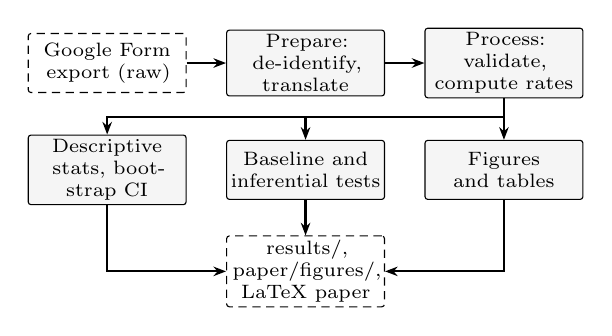
\begin{tikzpicture}[node distance=3.5mm and 5mm]
 \node[dat] (form) {Google Form export (raw)};
 \node[blk, right=of form] (prep) {Prepare: de-identify, translate};
 \node[blk, right=of prep] (proc) {Process: validate, compute rates};
 \node[blk, below=5.5mm of prep] (inf) {Baseline and inferential tests};
 \node[blk, left=of inf] (desc) {Descriptive stats, bootstrap CI};
 \node[blk, right=of inf] (viz) {Figures and tables};
 \node[dat, below=4.5mm of inf] (out) {results/, paper/figures/, LaTeX paper};
 \draw[arr] (form) -- (prep);
 \draw[arr] (prep) -- (proc);
 \draw[arr] (proc.south) -- ++(0,-2.4mm) -| (viz.north);
 \draw[arr] (proc.south) -- ++(0,-2.4mm) -| (inf.north);
 \draw[arr] (proc.south) -- ++(0,-2.4mm) -| (desc.north);
 \draw[arr] (desc.south) |- (out.west);
 \draw[arr] (inf.south) -- (out.north);
 \draw[arr] (viz.south) |- (out.east);
\end{tikzpicture}
\caption{Architecture of the analysis pipeline. Dashed boxes are data stores, solid boxes are scripts; all random steps use seed 42.}
\label{fig:arch}
\end{figure}

\section{Results and Discussion}
\label{sec:results}

\subsection{Experimental conditions and data quality}
All 17 respondents consented; none was excluded. Respondents were mostly third-year (11) or fourth-year (5) students, with one second-year student; tracks were cybersecurity (6), other IT (6), data/AI (3), networks (1), and software development (1). Seven reported professional experience and seven an internship (five reported both); five currently work in IT. No record violated the count rules and no value was missing. Six respondents sent no applications, so their rates are undefined and they enter only the perception analyses ($N=17$), whereas rate analyses use the $|\mathcal{A}|=11$ applicants. Two minor inconsistencies (three respondents chose more than three barriers; one reported not searching yet two applications) were retained and flagged.

\subsection{Baseline comparison}
Table~\ref{tab:results} compares applicants with internship experience against the baseline group without it; the corresponding distributions are shown in Fig.~\ref{fig:results}(a). Overall, applicants sent 65 applications and received 20 invitations and 12 offers, i.e.\ a pooled interview rate of 30.8\% (Wilson 95\% CI 20.9--42.8) and an offer rate of 18.5\% (10.9--29.6).

\begin{table}[t]
\centering
\caption{Internship group vs.\ baseline (no internship). Rates are percentages; intervals are Wilson 95\% CIs; IQR = interquartile range}
\label{tab:results}
\begin{tabular}{@{}lcc@{}}
\toprule
Indicator & Baseline & Internship \\
\midrule
Applicants / applications & 4 / 17 & 7 / 48 \\
Pooled interview rate & 17.6 (6.2--41.0) & 35.4 (23.4--49.6) \\
Median student rate [IQR] & 12.5 [0.0--27.1] & 26.7 [22.5--48.6] \\
Pooled offer rate & 11.8 (3.3--34.3) & 20.8 (11.7--34.3) \\
Applicants with $\ge 1$ offer & 2 / 4 & 5 / 7 \\
Working in IT now ($N{=}17$) & 1 / 10 & 4 / 7 \\
\midrule
Mean difference $\Delta$ [95\% CI] & \multicolumn{2}{c}{19.0 pp [$-2.6$, 39.5]} \\
$U$, $p$, $\delta$ (interview rate) & \multicolumn{2}{c}{20.5, 0.242, 0.46} \\
Fisher exact $p$ (working in IT) & \multicolumn{2}{c}{0.101 (odds ratio 12.0)} \\
\bottomrule
\end{tabular}
\end{table}

\begin{figure*}[t]
\centering
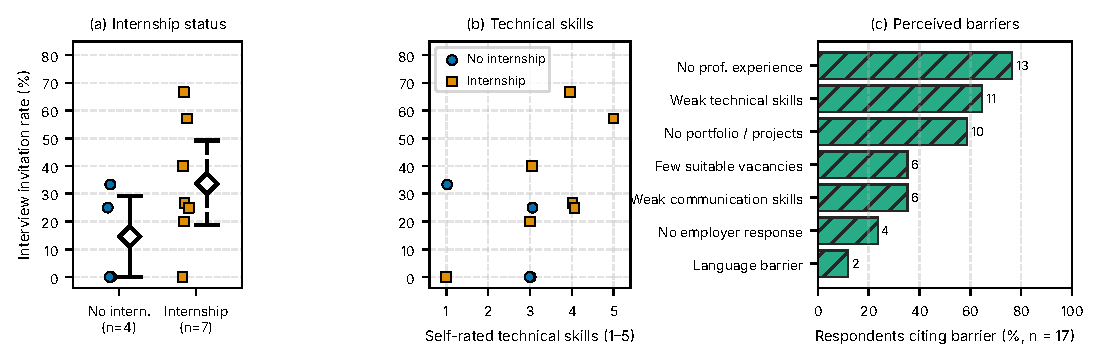
\includegraphics[width=\textwidth]{figures/fig_results.pdf}
\caption{Survey results. (a) Interview invitation rate by internship status (markers: students; diamonds: means with bootstrap 95\% CIs). (b) Interview rate against self-rated technical skills. (c) Share of all 17 respondents citing each barrier (counts at bar ends).}
\label{fig:results}
\end{figure*}

\subsection{Interpretation by research question}
Table~\ref{tab:tests} lists all tests: the three primary tests ($H_1$--$H_3$, Holm family) and six exploratory ones.

\begin{table}[t]
\centering
\caption{Hypothesis tests. $\delta$: Cliff's delta, $\rho$: Spearman's rank correlation, OR: odds ratio. Holm adjustment is applied to the primary tests only}
\label{tab:tests}
\footnotesize
\setlength{\tabcolsep}{3.5pt}
\begin{tabular}{@{}llcrcc@{}}
\toprule
ID & Contrast (outcome) & $n$ & Effect & $p$ & Holm $p$ \\
\midrule
$H_1$ & experience (difficulty) & 17 & $\delta=0.26$ & 0.378 & 0.485 \\
$H_2$ & internship (interview rate) & 11 & $\delta=0.46$ & 0.242 & 0.485 \\
$H_3$ & technical skills (interview) & 11 & $\rho=0.52$ & 0.103 & 0.309 \\
\midrule
$E_1$ & communication (interview) & 11 & $\rho=-0.37$ & 0.267 & --- \\
$E_2$ & projects (interview) & 11 & $\rho=-0.11$ & 0.738 & --- \\
$E_3$ & technical skills (offer) & 11 & $\rho=0.44$ & 0.179 & --- \\
$E_4$ & projects (offer) & 11 & $\rho=0.35$ & 0.296 & --- \\
$E_5$ & internship (offer) & 11 & $\delta=0.29$ & 0.485 & --- \\
$E_6$ & internship (working in IT) & 17 & OR$=12.0$ & 0.101 & --- \\
\bottomrule
\end{tabular}
\end{table}

\textit{RQ1.} Fig.~\ref{fig:results}(c) shows that missing professional experience (13 of 17), insufficient technical skills (11), and the lack of a portfolio or projects (10) were named most often, while language and employer non-response were rare. The top barriers resemble those that employers report for new graduates, notably missing project experience \cite{radermacher2014}, which suggests that students and employers perceive a similar gap, although our data cannot confirm that the perceived barriers are the actual causes of rejection. The median perceived difficulty was 4 on a five-point scale (mean 3.8; 59\% rated it 4 or 5). Respondents without experience did not rate the search as significantly harder than those with it (both medians 4; $\delta=0.26$, $p=0.378$, Holm-adjusted $p=0.485$), so $H_1$ is not supported in our data: the difficulty seems to be perceived broadly, regardless of experience.

\textit{RQ2.} Students with an internship reported roughly twice the pooled interview rate of the baseline (Table~\ref{tab:results}), and 4 of 7 interns currently work in IT versus 1 of 10 others. The direction agrees with résumé-audit evidence, although that design differs from ours in sampling, outcome definition, and randomisation, so the magnitudes are not comparable. Nevertheless, the bootstrap interval for $\Delta$ includes zero, the Wilson intervals overlap, and the adjusted $p$-value is 0.485. The employment contrast is also partly circular, because an internship may itself be the current position. The number of projects was not associated with the interview rate ($\rho=-0.11$, $p=0.738$, exploratory).

\textit{RQ3.} Self-rated technical skills showed a moderate positive rank correlation with the interview rate ($\rho=0.52$, $n=11$, raw $p=0.103$, Holm-adjusted $p=0.309$; Fig.~\ref{fig:results}(b)), whereas communication skills showed a weak negative one ($\rho=-0.37$, $p=0.267$, exploratory). Dropping each applicant in turn leaves the signs unchanged (leave-one-out $\rho$ between 0.37 and 0.74 for technical and between $-0.63$ and $-0.21$ for communication skills), so the direction seems stable although its magnitude is imprecise. Self-assessments are also known to be biased. These results suggest, but do not demonstrate, a role of technical skills.

\textit{Practical implications.} Three of the four most frequent barriers (experience, portfolio, technical skills) can partly be addressed by project courses and structured internships. If the internship contrast replicated in a larger sample, it would be consistent with internships acting as an employer signal; at present this remains conjectural, since self-selection of stronger students cannot be ruled out.

\section{Limitations and Conclusion}
\label{sec:conclusion}

\subsection{Threats to validity}
\textit{Internal:} the design is observational; students with internships may also have higher skills, motivation, or more applications, and no confounder was adjusted for. \textit{Construct:} skills and difficulty are self-reported single items; ``internship'' and ``working in IT'' overlap; the barrier question allowed more than three answers in three cases. \textit{External:} the sample is a small convenience sample, probably dominated by third-year cybersecurity and ``other IT'' students from similar networks, so generalisation is unwarranted. \textit{Statistical conclusion:} with $N=17$ and $|\mathcal{A}|=11$, power is low, intervals are wide, and non-significance is not evidence of no effect; Wilson intervals ignore within-student clustering.

\subsection{Conclusion and future work}
Within our experimental setup, the research questions can be answered as follows. \textbf{RQ1:} perceived barriers centred on missing experience, technical skills, and portfolios, and difficulty was rated high irrespective of experience ($H_1$ not supported). \textbf{RQ2:} internship experience was directionally associated with a higher interview rate and with current IT work, whereas the number of projects was not; the primary test was nevertheless not significant ($H_2$ not supported at $\alpha=0.05$). \textbf{RQ3:} technical skills were moderately and positively associated with the interview rate, communication skills were not; again, the Holm-adjusted $p$-value exceeded 0.30 ($H_3$ not supported). The contribution is thus a reproducible baseline with effect-size estimates, not a confirmed effect.

Future work should (i) recruit a larger, multi-institution sample with a pre-registered target size, (ii) model outcomes with count regression adjusted for applications, year, and track, (iii) validate self-rated skills against objective assessments, and (iv) follow students longitudinally to separate the effect of an internship from selection into it.

\balance
\bibliographystyle{IEEEtran}
\bibliography{references}

\end{document}
